\chapter{Overview}
\label{Chapter1}
\lhead{Chapter 1. \emph{Overview}}

In almost all modern portable consumer devices, Bluetooth plays a large role; it is available in the vast majority of mobile phones and their associated accessories, in cars, in laptops and, most recently, in mobile tablet PCs. Bluetooth as a technology gives a standardized low power wireless communications standard from the baseband up to the higher level services, allowing implementing devices to communicate with one another in a manufacturer-agnostic way. This freeing of consumers from the proprietary short range wireless solutions (such as \textit{ZigBee}) has helped make Bluetooth the wireless communication system of choice for many applications.

\section{Project Background}

Despite this ubiquity, Bluetooth remains firmly in the realm of systems containing large amounts of RAM, storage, processing power and - in many cases - full operating system stacks. For small-scale embedded devices with tiny 8-bit processors, clock speeds in the tens of MHz (or even less) and RAM measured in kilobytes, Bluetooth remains impractical either due to its expense or the lack of suitable software.

However, existing solutions do exist. System designers can integrate off-the-shelf Bluetooth solutions in their products; small hardware modules containing the Bluetooth baseband and a fixed-function microprocessor, which handles the complex onion-like layers of the various Bluetooth stack components. These modules are generally fixed function however, making them unsuitable in applications where a specific or even custom Bluetooth service is required. In addition, such modules are generally significantly more expensive than the product's main processor, negating its cost/benefit ratio where a more powerful system processor could be substituted to manage the entire application including the Bluetooth component.

These turn-key modules are made all the less attractive when one considers the cost of a raw Bluetooth baseband IC module, without an integrated processor to manage the software stack; these are generally available from multiple vendors at costs measured in the sub-US\$5 range. This indicates that the main cost of the complete modular solutions lies not in the physical hardware, but the IP of the Bluetooth software stack. If such a stack could be made widely available for use in embedded systems, this fixed-cost vendor lock-in could be avoided and cheaper Bluetooth enabled systems developed for both hobbyist and commercial use.

\section{Project Brief}

To help fill this gap in the marketplace for a cheap, open source Bluetooth stack aimed at the low to mid-range embedded market, it is proposed that a new stack be designed from scratch specifically for this market segment. This stack would offer a base amount of functionality suitable for integration into new or existing embedded systems, to extend the system functionality to include wireless Bluetooth communications.

At a minimum, a functional Bluetooth stack needs to have at least four components:

\begin{enumerate}
	\item A \textbf{Physical Data Transport layer} to and from a connected Bluetooth physical baseband tranciever IC
	\item An implementation of the Bluetooth specification's \textbf{HCI layer} for the establishment and management of physical connections to and from remote devices
	\item An implementation of the Bluetooth specification's \textbf{L2CAP layer} for the establishment and management of logical channels within an established connection
	\item One of more \textbf{Bluetooth Services} on top of the L2CAP layer to implement functionality such as the Service Discovery Protocol (SDP)
\end{enumerate}

These components, when put together, form the basis of a minimal Bluetooth stack \emph{(see Figure \ref{fig:btstack})}. Additional services may or may not be added on top of the stack in parallel with the mandatory SDP protocol to expose local device functionality and interact with remote devices.

\begin{figure}[H]
	\centering
		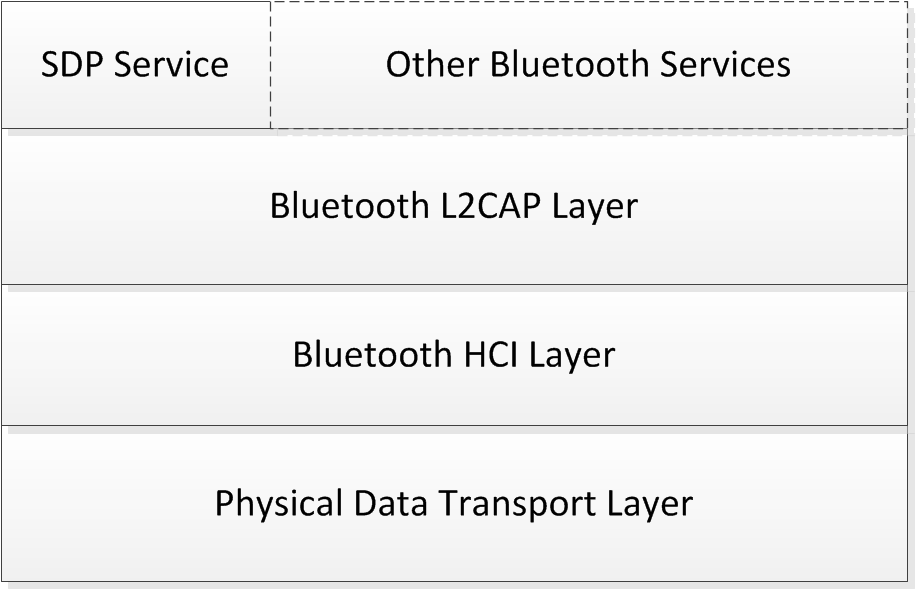
\includegraphics[width=80mm]{./Figures/BluetoothStack.png}
	\rule{35em}{0.5pt}
	\caption[Diagram of a typical Bluetooth Stack]{Diagram of the basic components which form a typical Bluetooth Stack}
	\label{fig:btstack}
\end{figure}

As the usefulness of an abstract piece of software is inherrantly low without a suitable demonstration platform, a second component of the project will be to design, develop and prototype a functional and practical device which uses the created stack. It is proposed that this hardware component be in the form of a small \textit{"ExplorerBot"} robot, able to stream local sensor data wirelessly to a remote PC for real-time graphing purposes, and to allow for remote wireless control over a Bluetooth link to a consumer Bluetooth control device - such as a current generation Game Console controller (\textit{Wii} or \textit{Playstation 3}). If possible, these two functions should be combined to allow for multiple simultaneous connections, allowing for remote control at the same time as the sensor data is logged remotely.

% TODO - Figure of robot

With the combination of the software \emph{(the stack)} and hardware \emph{(the robot)} components of this project, the final design should offer a complete system and test platform which can be reproduced wholesale, modified to suit a particular application or used as a reference implementation for other projects.

\section{Design Goals}

The design goals of the project were split into two parts \emph{(software and hardware)} in order to seperate the testing platform hardware goals from those of the logical Bluetooth stack.

\subsection{Software Goals}

For such a stack to be useful in an embedded environment, it must be able to conform to the restrictions such an environment imposes. Specfically, the completed stack must minimize its compiled and working set footprints, reduce or eliminate the need for dynamic memory allocation, and minimize its hardware dependencies to suit as wide a range of processors of differing capabilities as possible.

The design goals of the complete software stack were therefore set to:

\begin{itemize}
	\item Use as little RAM as possible
	\item Compile to as small a binary as is practical
	\item Offer a framework upon which services can be added to suit a particular application
	\item Provide asynchronous events to which the user application can respond to
	\item Allow for a variable number of simultaneous connections and logical channels to/from remote devices
	\item Have no requirement for dynamic memory allocation on the heap
	\item Be fully decoupled from the physical transport to the Bluetooth Adapter
	\item Be endian-correct regardless of native processor endianness
\end{itemize}

\subsection{Hardware Goals}

To make a useful, visual and functional testing platform, a decision was made to produce a small, battery powered robot. This robot would serve as a both a testing platform for the completed stack to verify its correct operation in a real-world environment during development, and to function as a reference application of the completed stack.

In order to fully demonstrate the capabilities of the Bluetooth stack, the robot would have to include both locally initiated Bluetooth connections, as well as accept remotely initiated connections. In addition, data would have to be both received and processed by the device, as well as sent to a remote device.

A set of design goals was thus created for the robot:

\begin{itemize}
	\item Allow the user to initiate a connection to a remote device via the robot
	\item Accept incoming connections from remote Bluetooth devices, including authentication
	\item Consume data received from remote Bluetooth device(s) via one or more Bluetooth services
	\item Produce data to be transmitted to remote Bluetooth device(s) via one or more Bluetooth services
	\item Visually indicate status and debug messages via a display mechanism, for debugging
	\item Allow for the robot to be remotely driven via a set of PWM controlled DC motors
\end{itemize}

% TODO
